\documentclass[
	%a4paper, % Use A4 paper size
	letterpaper, % Use US letter paper size
]{jdf}
\usepackage{graphicx}
\usepackage{float}
\addbibresource{references.bib}


\author{Ali El-Khatib}
\email{aelkhatib6@gatech.edu}
\title{Homework 1}

\begin{document}
\maketitle
\section{Question 1}
\subsection{Star Wars Semantic Network}
\begin{figure}[H]
	\centering
	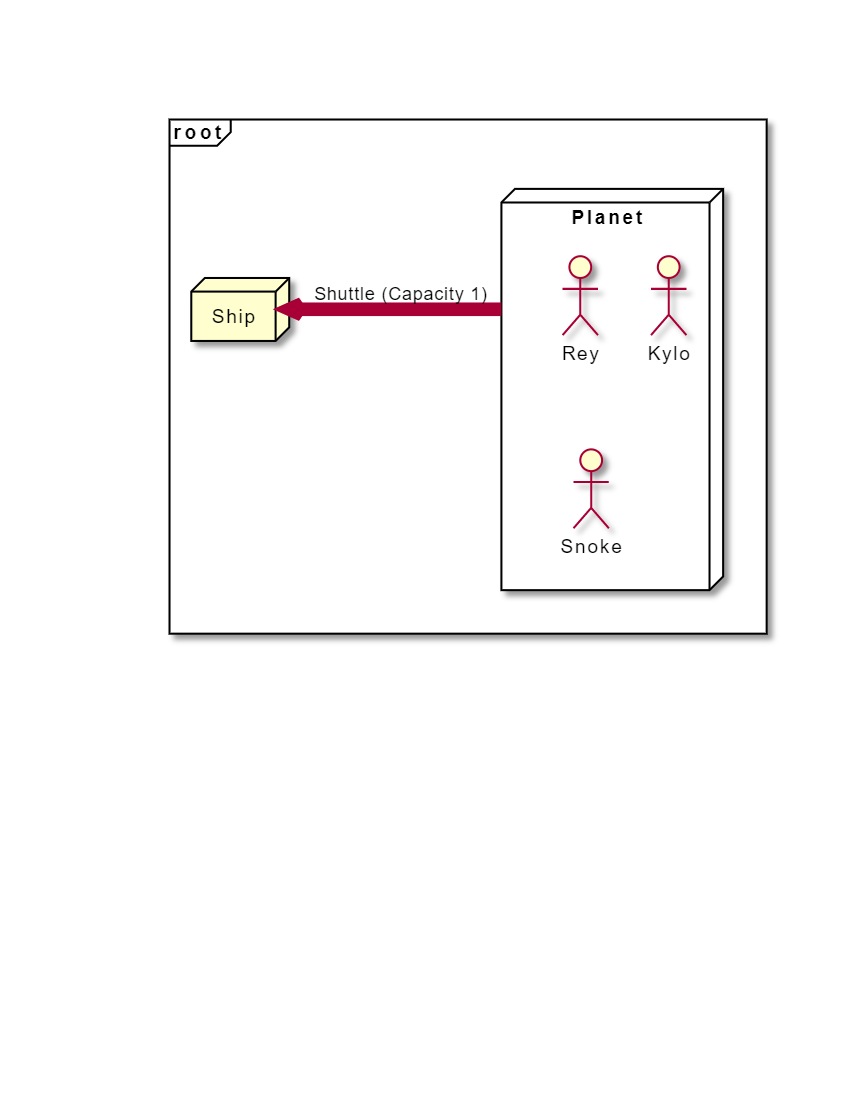
\includegraphics[width=0.7\linewidth]{../figures/starwars-semantic-network}
	\caption{Semantic Network representation of the Star Wars-themed river crossing problem}
	\label{fig:starwars-semantic-network}
\end{figure}
\pagebreak
\subsection{Generate \& Test}
\begin{figure}[hbtp]
	\centering
	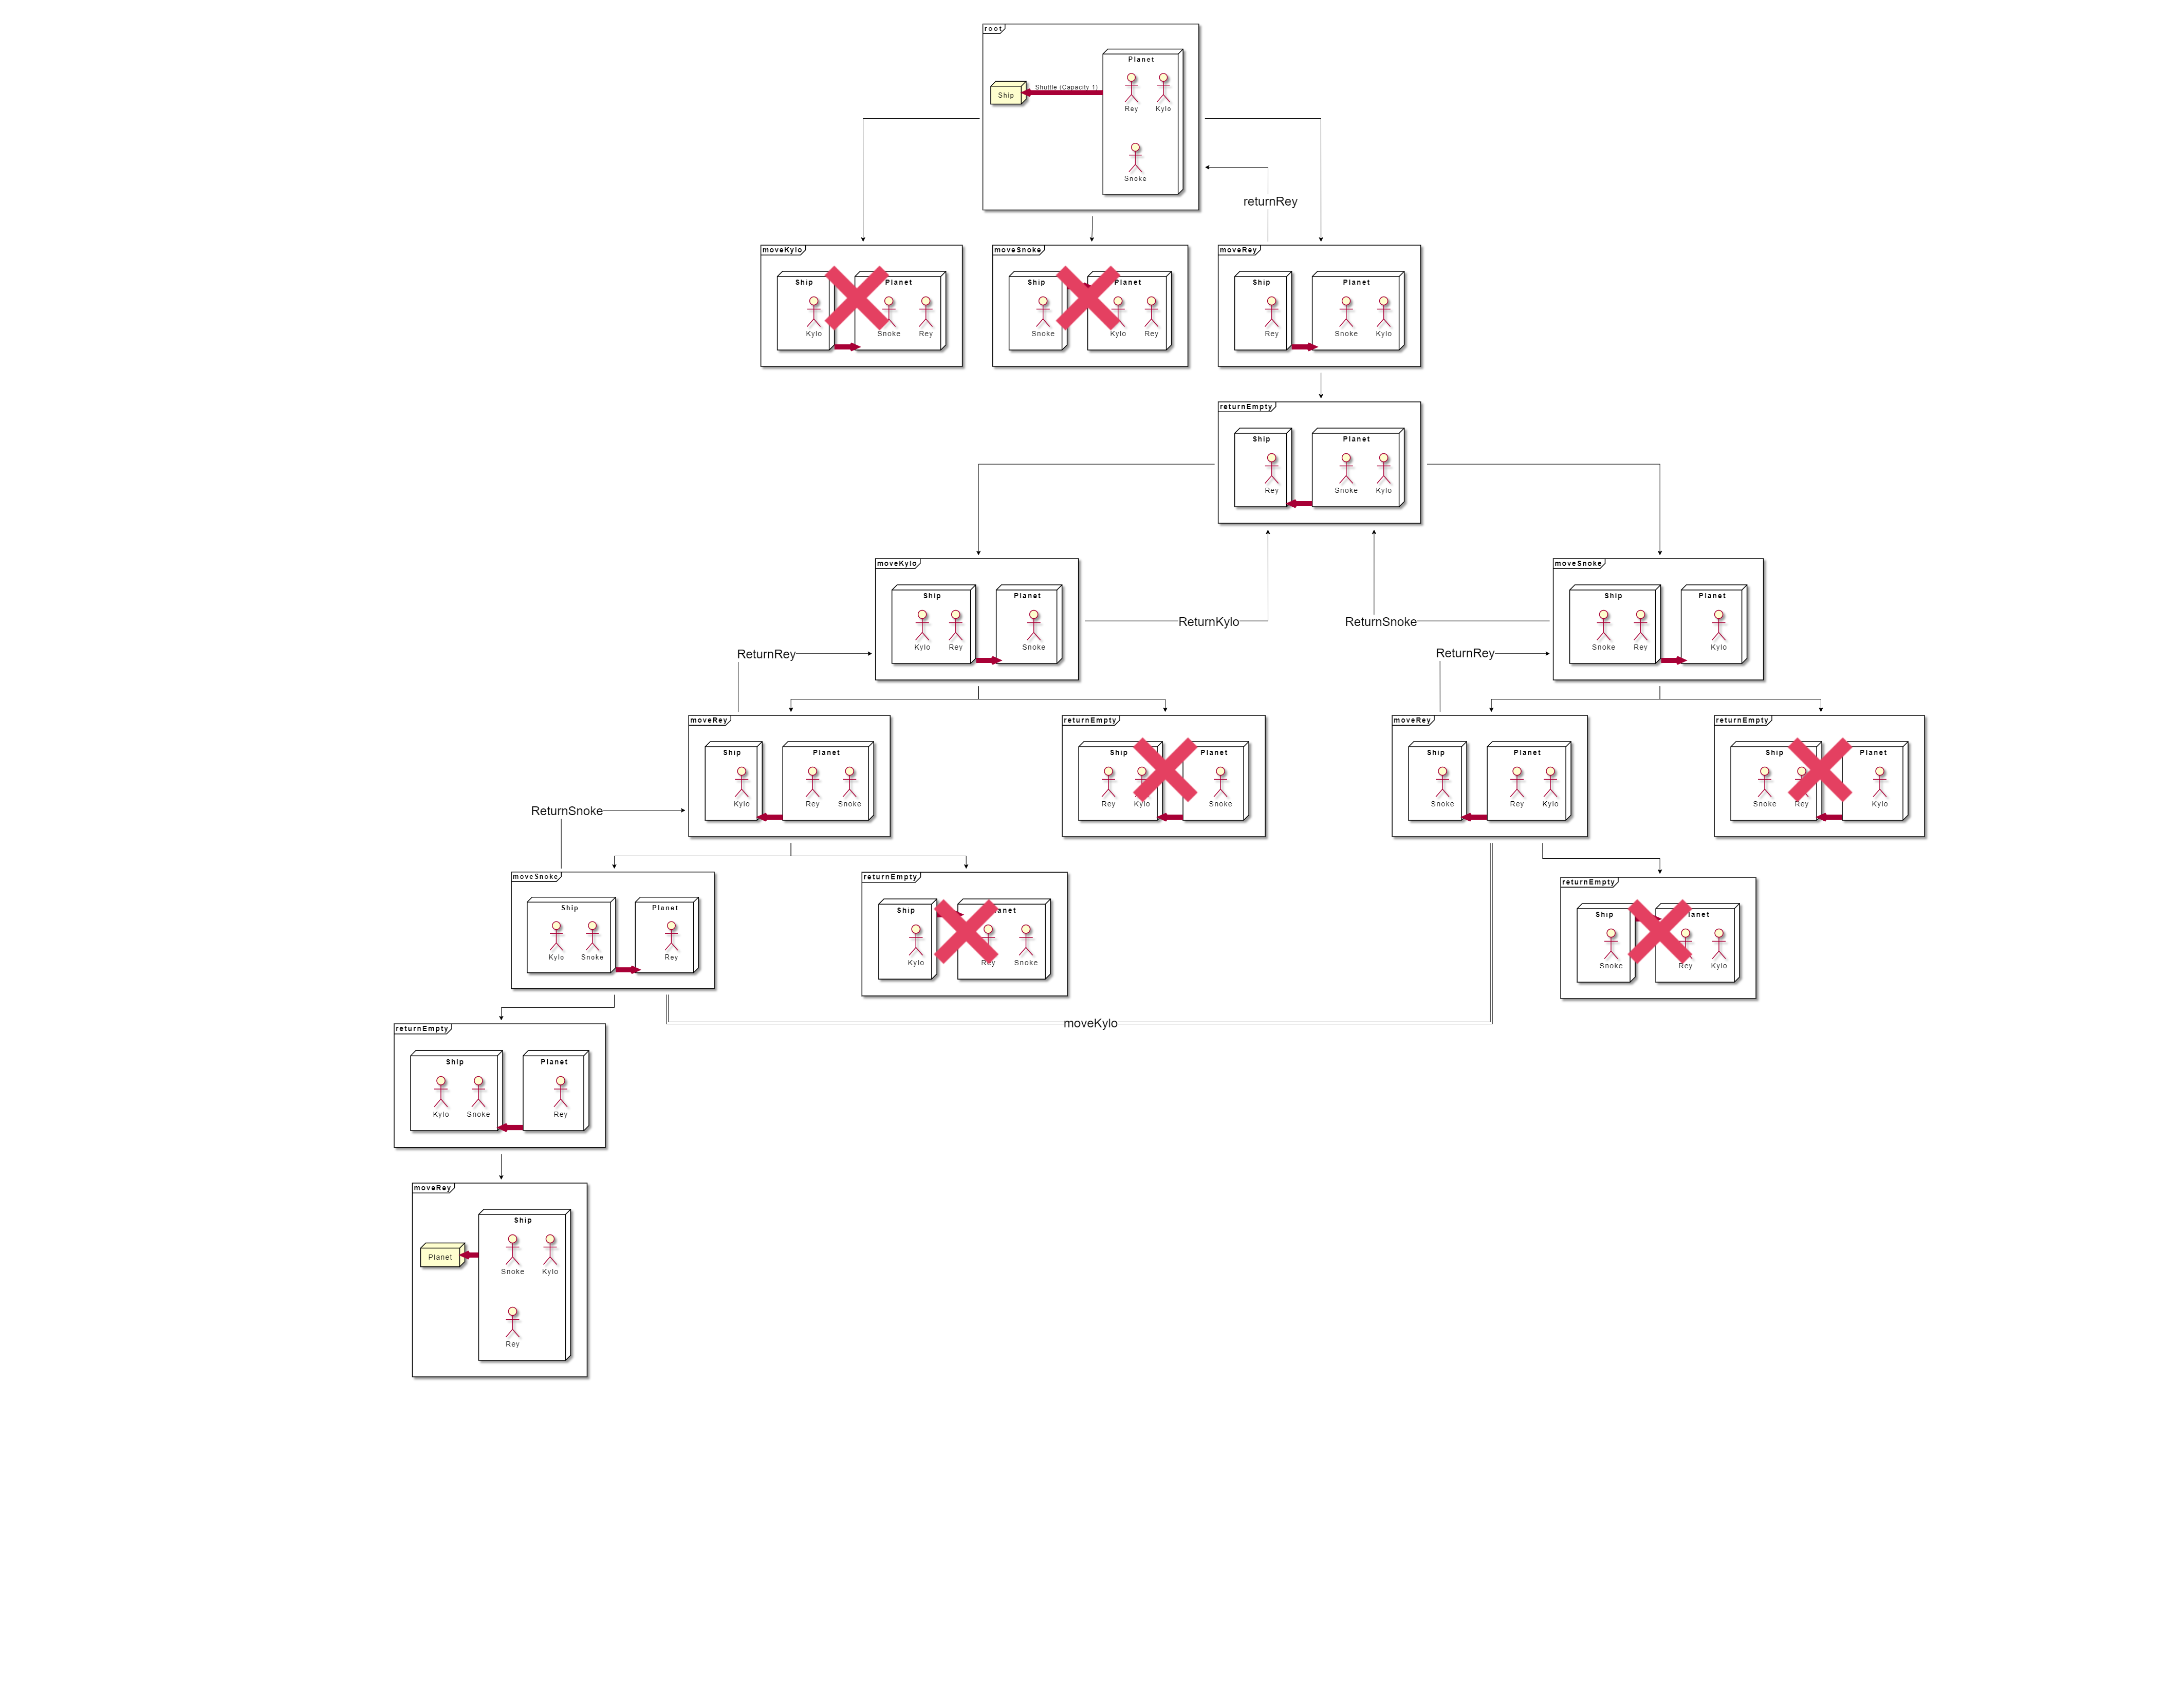
\includegraphics{../figures/semantic-network-Page-1.drawio}
	\caption{State transitions for solution to semantic network problem posed in  Figure \ref{fig:starwars-semantic-network}}
	\label{fig:semantic-network-page-1}
\end{figure}
\pagebreak



\section{Question 2}
\subsection{General Data Protection Regulation \& You}
The General Data Protection Regulation (GDPR) --adopted on April 27, 2016-- is a regulation regarding the protection of personal data and privacy. In effect, it allows users within Europe to have increased control of all personal data (e.g., website cookies, email addresses, phone number). This means that users control the activation of cookies and trackers--methods which collect personal data--on websites they visit. In addition to data control, it enforces a number of other rights for users:
\begin{itemize}
	\item Right of an individual to be free of inaccurate personal data (\href{https://gdpr-info.eu/art-16-gdpr/}{Article 16})
	\item Right to be erasure (or forgotten); ability to have data deleted upon request (\href{https://gdpr-info.eu/art-17-gdpr/}{Article 17})
	\item Right to have data provided in portable, standardized formats (e.g., .csv, .xlsx) (\href{https://gdpr-info.eu/art-20-gdpr/}{Article 20})
	\item Right to refuse their data being used in certain processes (\href{https://gdpr-info.eu/art-18-gdpr/}{Article 18}, \href{https://gdpr-info.eu/art-21-gdpr/}{Article 21})
	\item Right to not have decisions based solely on automated processes (\href{https://gdpr-info.eu/art-22-gdpr/}{Article 22})
\end{itemize}


The GDPR applies in both European Union (EU) member states and the European Economic Area (EEA), both of which are illustrated in Figure~\ref{fig:europe-groups}. The EEA extends the single-market of the EU to other member states within the European Free Trade Association (i.e., Iceland, Liechtenstein, and Norway) \href{https://www.efta.int/eea/eea-agreement/eea-basic-features#1}{\cite{efta}}.
\begin{figure}[H]
	\centering
	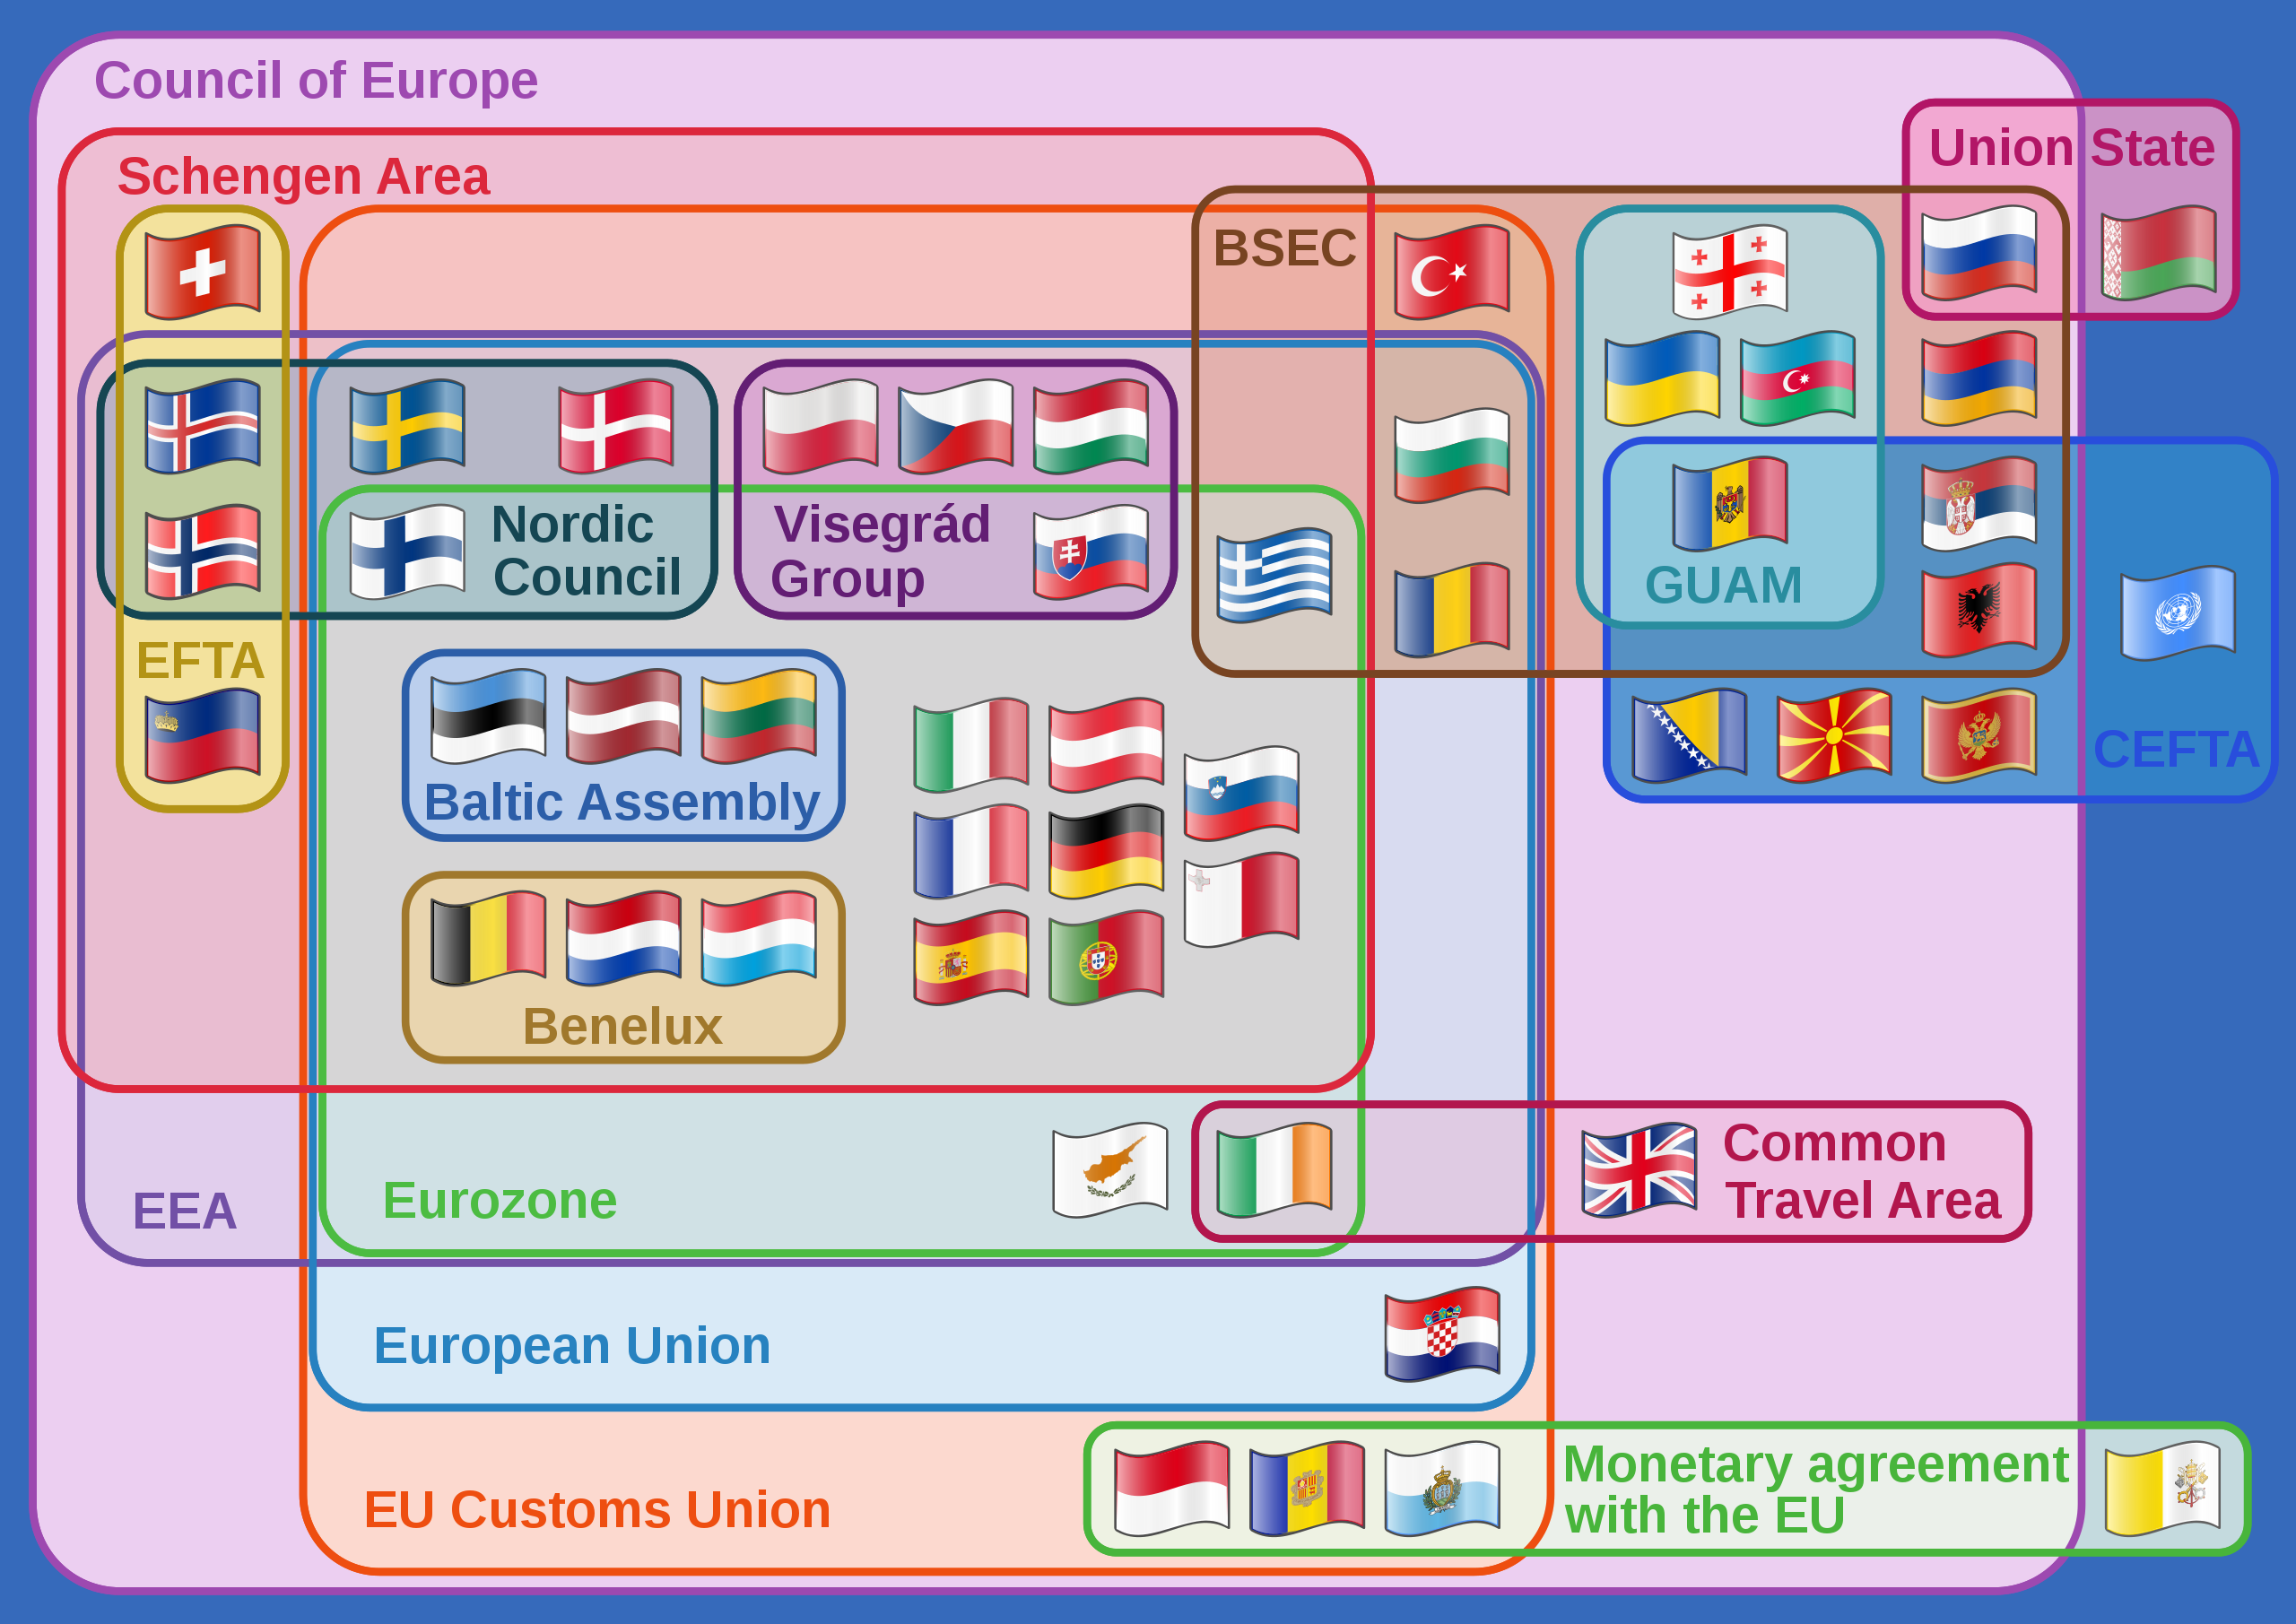
\includegraphics[width=0.7\linewidth]{../figures/europe-groups}
	\caption{Euler Diagram illustrating the various multinational European organizations and agreements. European Union is shown in light blue; EEA is in purple. Source: \href{https://en.wikipedia.org/wiki/File:Supranational_European_Bodies-en.svg}{Wikipedia}
	}
	\label{fig:europe-groups}
\end{figure}



\subsection{The Case of Google Advertising}
An easily accessible example of the impact of GDPR is Google's Ad personalization, which provides a major revenue source for many websites as well as Google itself. As a result of the GDPR, Google now allows individuals to view the data that is being used to target ads specifically to them. At this moment, anyone with a Google account can go to \href{https://adssettings.google.com/}{Google Ad Settings} and view the process behind Google's ad personalization, shown in \ref{fig:google-ads}. Additionally, it allows the selective removal of an individual's personal info as well as toggling off Ad personalization. Without the usage of AI algorithms in its infancy, Google's established reputation as a leader in web-indexing and advertising would have been overtaken by another innovative company. 

\begin{figure}
	\centering
	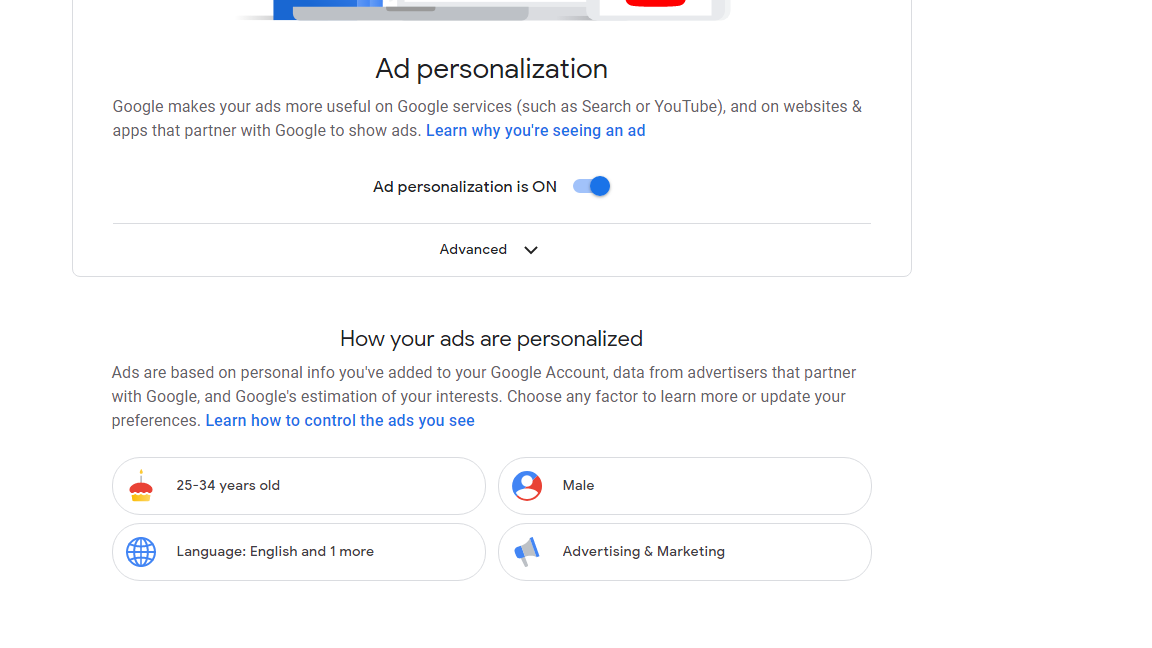
\includegraphics[width=0.7\linewidth]{../figures/google-ads}
	\caption{Example of data Google uses to target ads towards myself (the author)}
	\label{fig:google-ads}
\end{figure}


To comply with GDPR--to the best of my knowledge--, Google has completed the following:
\begin{itemize}
	\item Modifying or correcting personal data (\href{https://gdpr-info.eu/art-16-gdpr/}{Article 16}),
	\item Complete deletion of personal data and accounts (\href{https://gdpr-info.eu/art-17-gdpr/}{Article 17})
	\item Allowed toggling off ad personalization (\href{https://gdpr-info.eu/art-18-gdpr/}{Article 18},  \href{https://gdpr-info.eu/art-21-gdpr/}{Article 21}, \href{https://gdpr-info.eu/art-22-gdpr/}{Article 22} )
\end{itemize}
As a result of the GDPR, targeted advertising is still completed possible with only the consent of the users. Without being able to target potential markets, I would suspect that advertising would follow a more random approach, or more reasonably use third-party data such as a website's intended or suspected audience to control the ads shown. Though, this could lead to pervasive techniques such as virtual or physical geofencing marketing.

\subsection{No GDPR, No Service}
Clearview AI is a private American company specializing in facial recognition software, and caters to businesses, governmental agencies, and individuals, although explicitly mentioning only law enforcement agencies \cite{g2e}.   
Clearview AI's questionable practices involved scraping social media sites for user images and subsequently using those images in their AI software \cite{hill_secretive_2020}. This is in massive violation of the GDPR regulations mentioned above, and this has resulted in numerous government mandates for the company to delete its facial recognition data within Europe \cite{brandom_french_2021}, as well as Australia \cite{australia}. The company does not seem to be tenable, at least within Europe and even Australia. Their main product would require millions of individuals to waive their GDPR rights in order to be useful. In absence of these waivers, their facial recognition software would most likely not be of use due to lack of training data. 

\printbibliography
\end{document}